\documentclass{article}
\usepackage{a4wide}


\usepackage{polski}
\usepackage[utf8x]{inputenc}
\usepackage{graphicx}
\usepackage{float}
\usepackage{hyperref}
\usepackage{listings}
\usepackage{mathtools}
\usepackage{amsmath}

\usepackage{color} %red, green, blue, yellow, cyan, magenta, black, white
\definecolor{mygreen}{RGB}{28,172,0} % color values Red, Green, Blue
\definecolor{taupe}{rgb}{0.28, 0.24, 0.2}
\definecolor{mylilas}{RGB}{0,110,0}


\author{Lev Sergeyev}
\title{SPC. Ćwiczenie 3. Układy Automatycznej Regulacji}

\date{22.11.2019, pt/TN 13:15}
\begin{document}

\maketitle

%\pagebreak


\section{Regulator P}
\par
Dany obiekt:
\begin{equation}
K_O(s)=\frac{1}{(s+1)^3} 
\end{equation}

Za pomocą narzędzia Simulink stworzono układ automatycznej regulacji z regulatorem typu P \( (K_{r}(s) = k ) \) podanego obiektu(dodano sprzężenie zwrotne i wzmocnienie k).
Następnie przeprowadzono symulację odpowiedzi \(Y\) i uchybu \(E\) na skok w chwili \(t_0 = 0\) dla róźnych k:
\begin{figure}[h]
\centering
\scalebox{0.25}{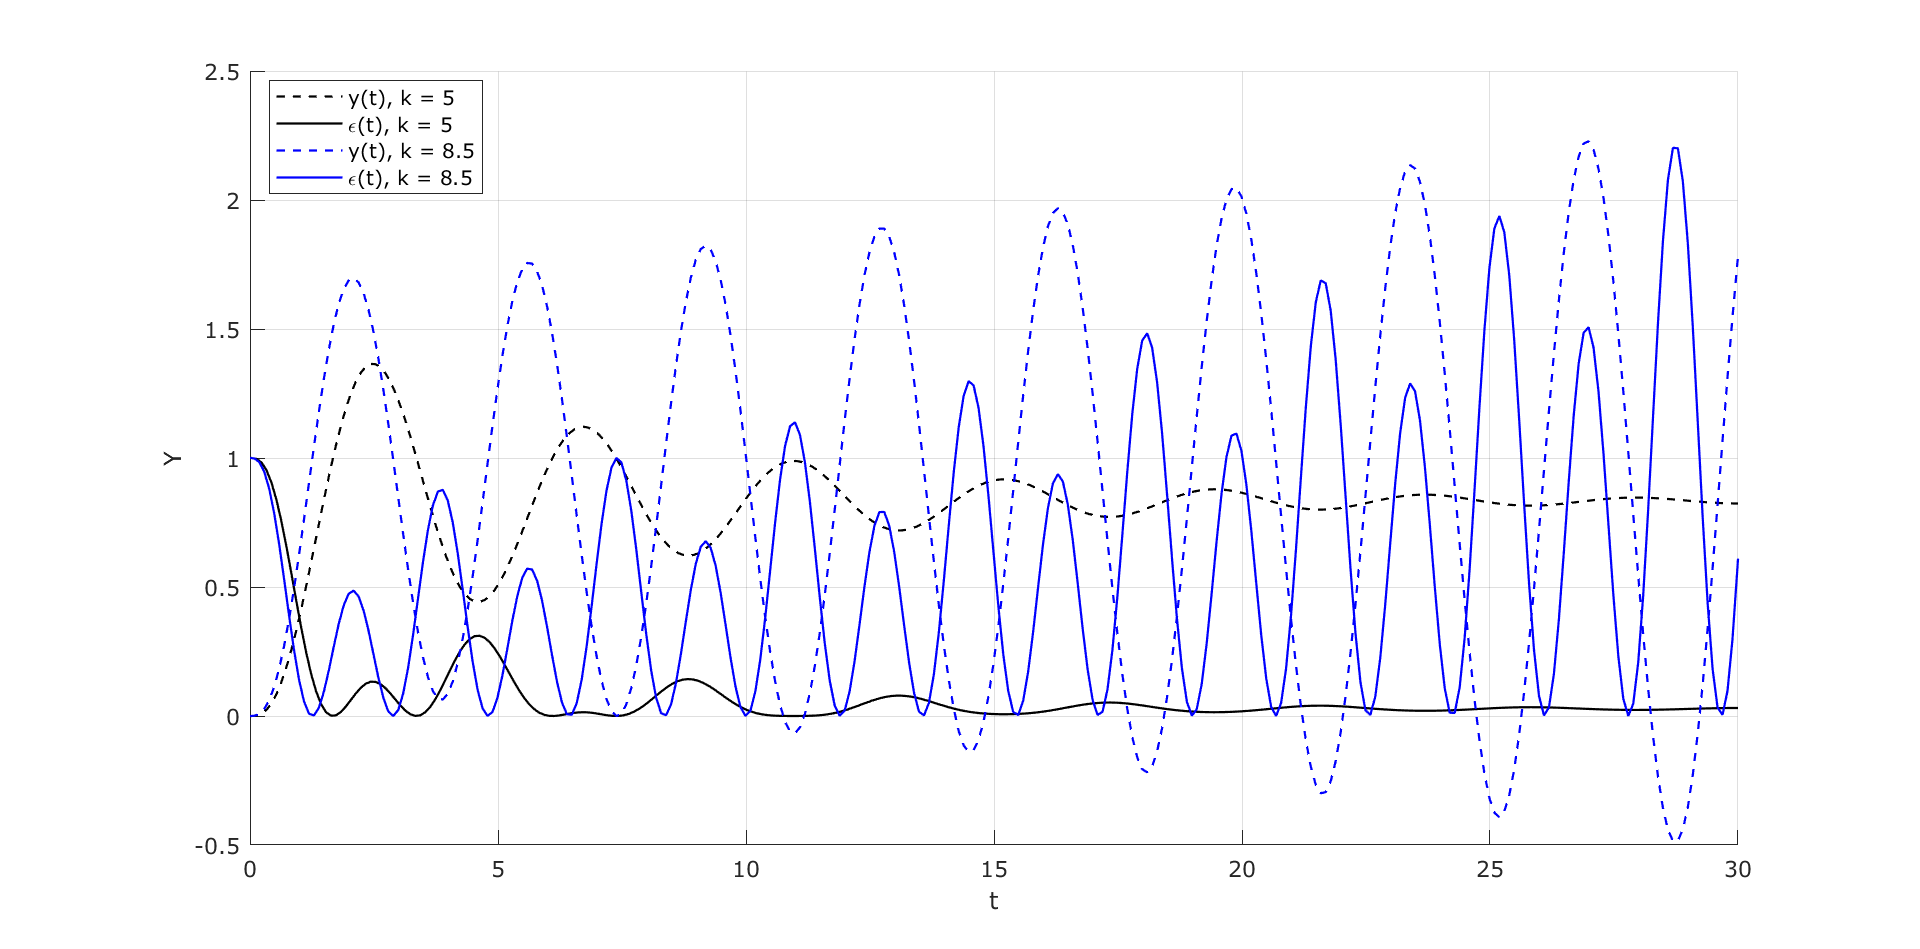
\includegraphics{1.png}}
\caption{Odpowiedź na skok układu z regulutaorem P dla róźnych \(k\)}
\end{figure}

%\pagebreak

\section{Regulator PI}

Dokonano zmiany regulatora z P na PI (dodano część całkującą \(\frac{k_2}{s} \) ), \(K_{r}(s) = k+ \frac{k_2}{s} \). Dalej przyjęto, że \(k\) jest stałe i \(k = 5\).

\subsection{Dobór nastaw}
Przeprowadzono symulację (Rys. 2) dla róźnych \(k_2\), dla każdej symulacji zmierzono całkę kwadratu uchybu \( Q = \int_{0}^{100} \epsilon(t)^2  dt\) 

\begin{figure}[h]
\centering
\scalebox{0.15}{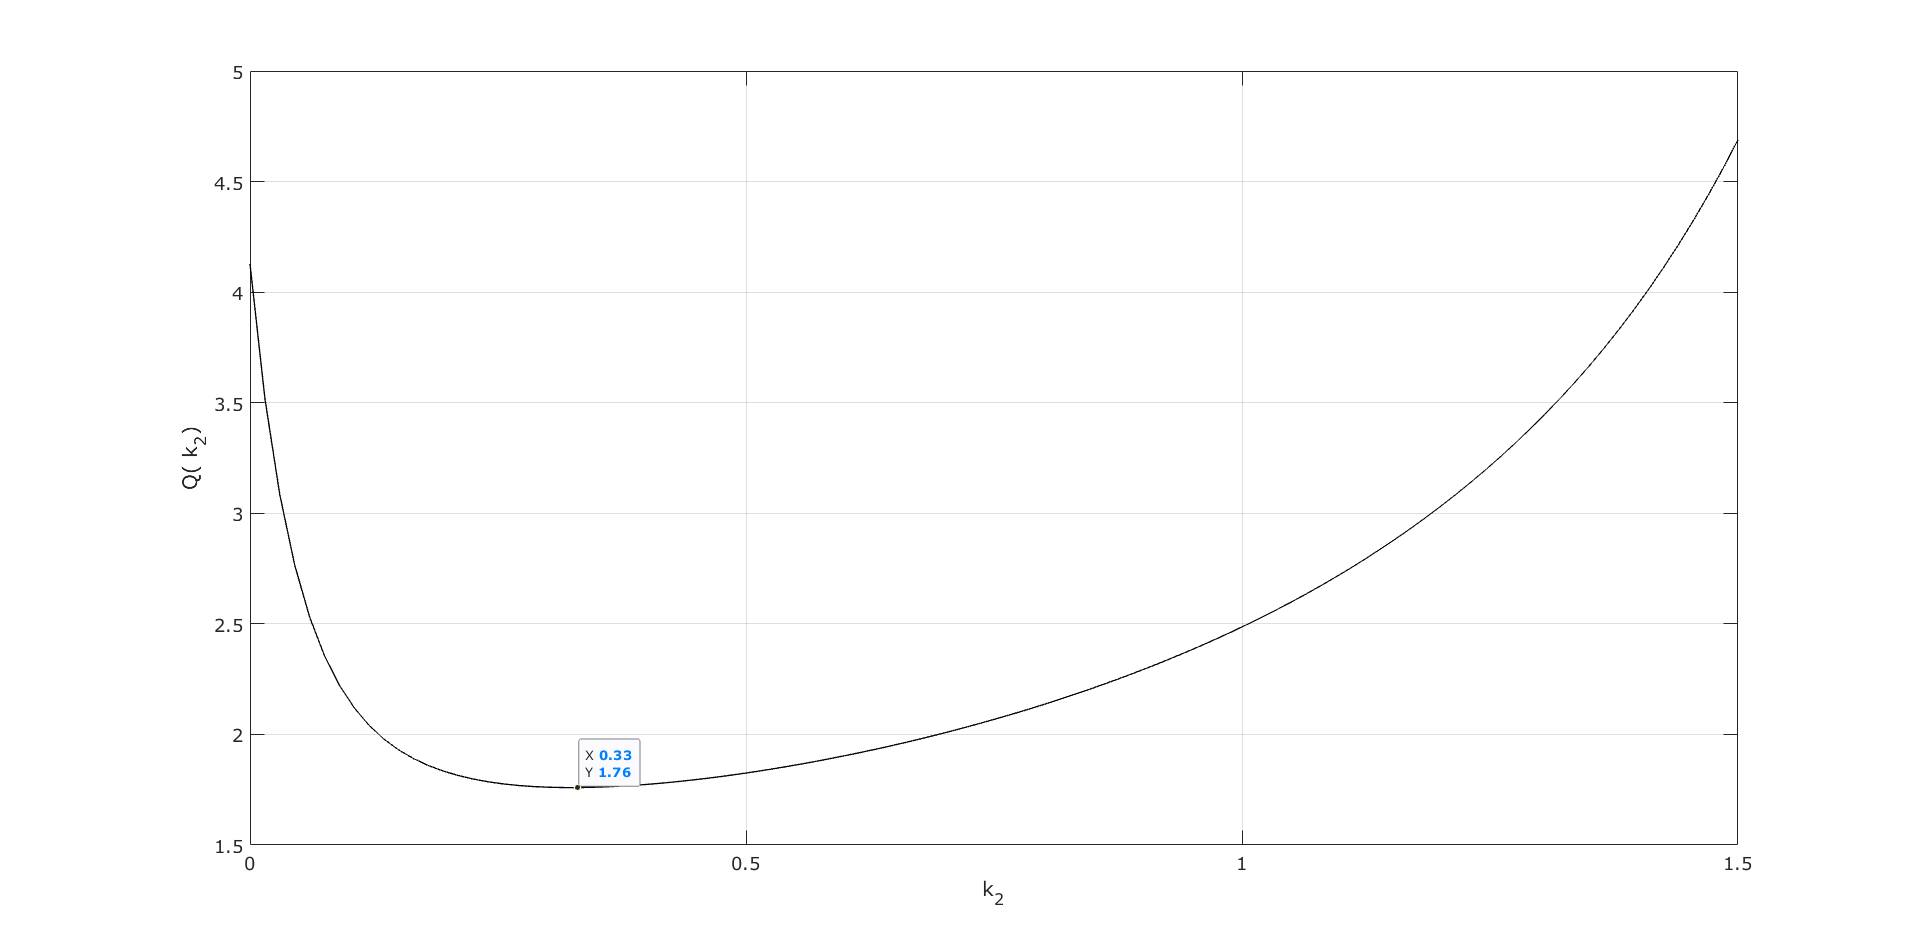
\includegraphics{2.png}}
\caption{Zależność \( Q \) od \(k_2\)}
\end{figure}

\pagebreak
Z rysunku widać, że regulacja jest optymalna dla \( k_2 = 0.33 \), wtedy \(Q\) jest minimalne.

\subsection{Porównanie odpowiedzi}

\begin{figure}[ht]
\centering
\scalebox{0.15}{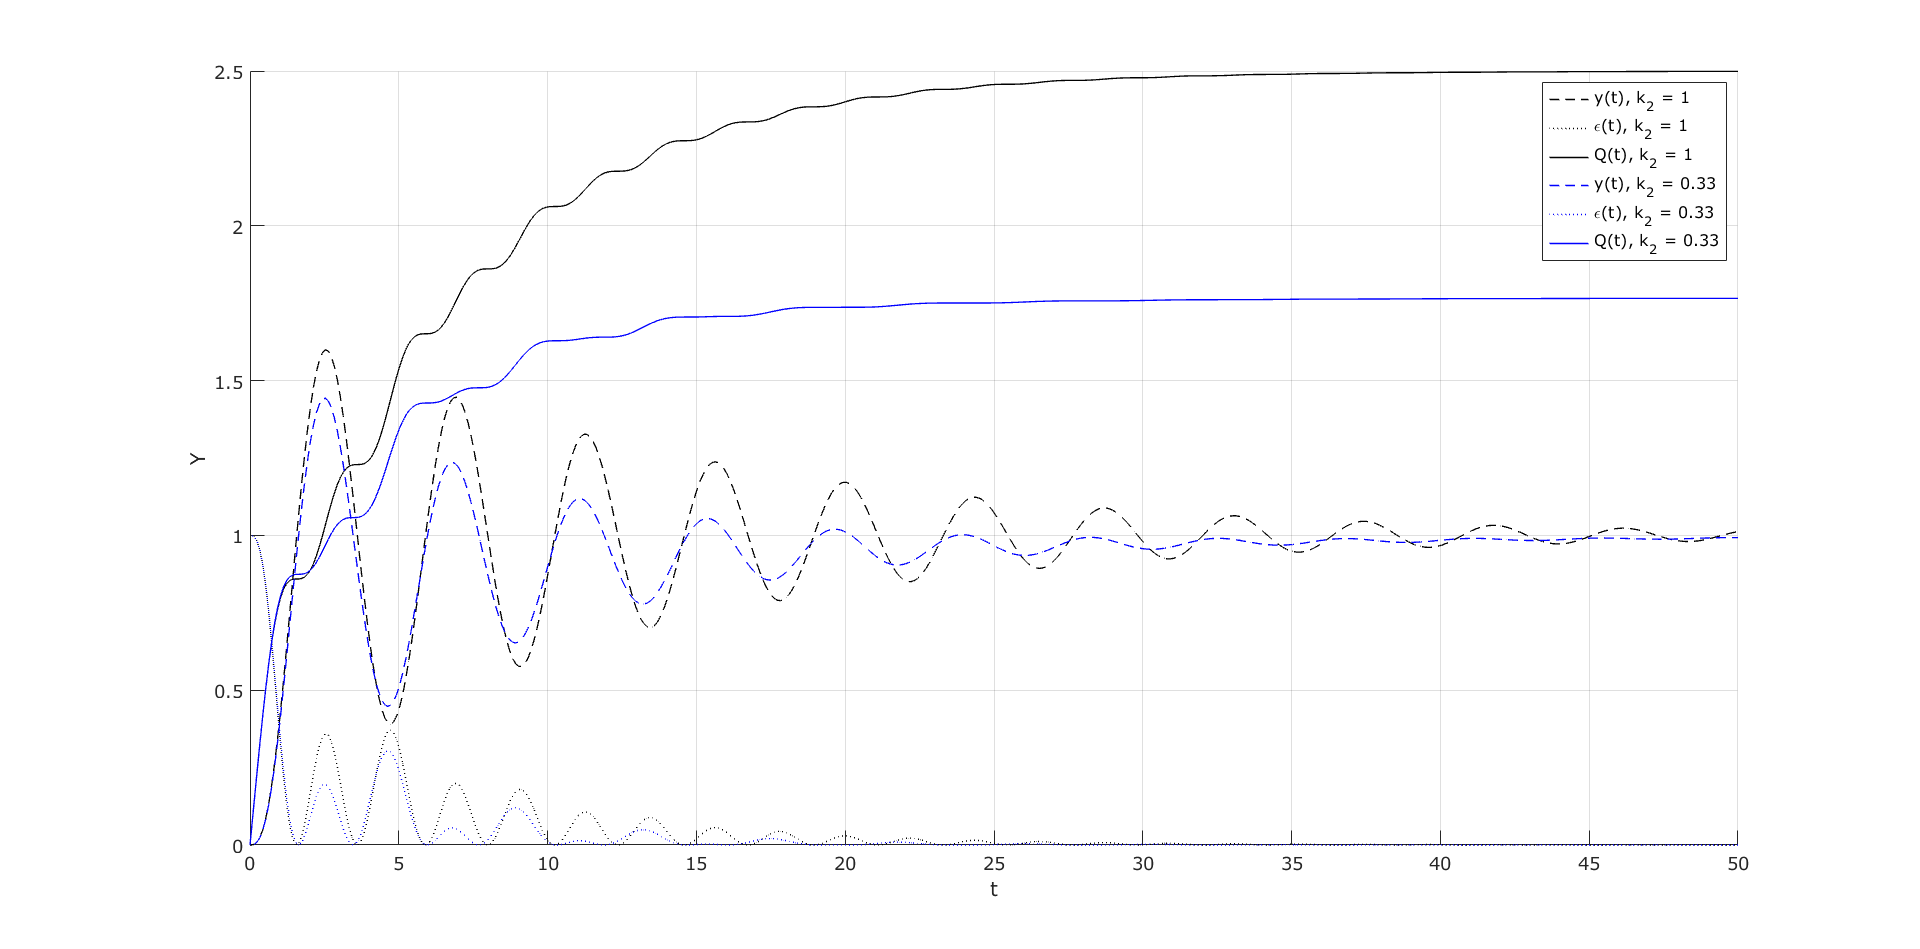
\includegraphics{2_1.png}}
\caption{Odpowiedź UAR na skok dla róźnych \(k_2\)}
\end{figure}


\section{Dyskretny regulator PI}

\subsection{Dyskretyzacja}

Przejście na postać dyskretną regulatora PI, \(K_R(s) \rightarrow K_R(z) \):

\begin{equation}
K_R(z)=\frac{z-1}{z} Z \left[ \frac{K_R(s)}{s} \right] = \frac{z-1}{z} (\frac{kz}{z-1}  + \frac{k_2 T_d z}{(z-1)^2}) = \frac{kz + k_2 T_d - k}{z-1} 
\end{equation}

\pagebreak
\begin{figure}[ht]
\centering
\scalebox{0.15}{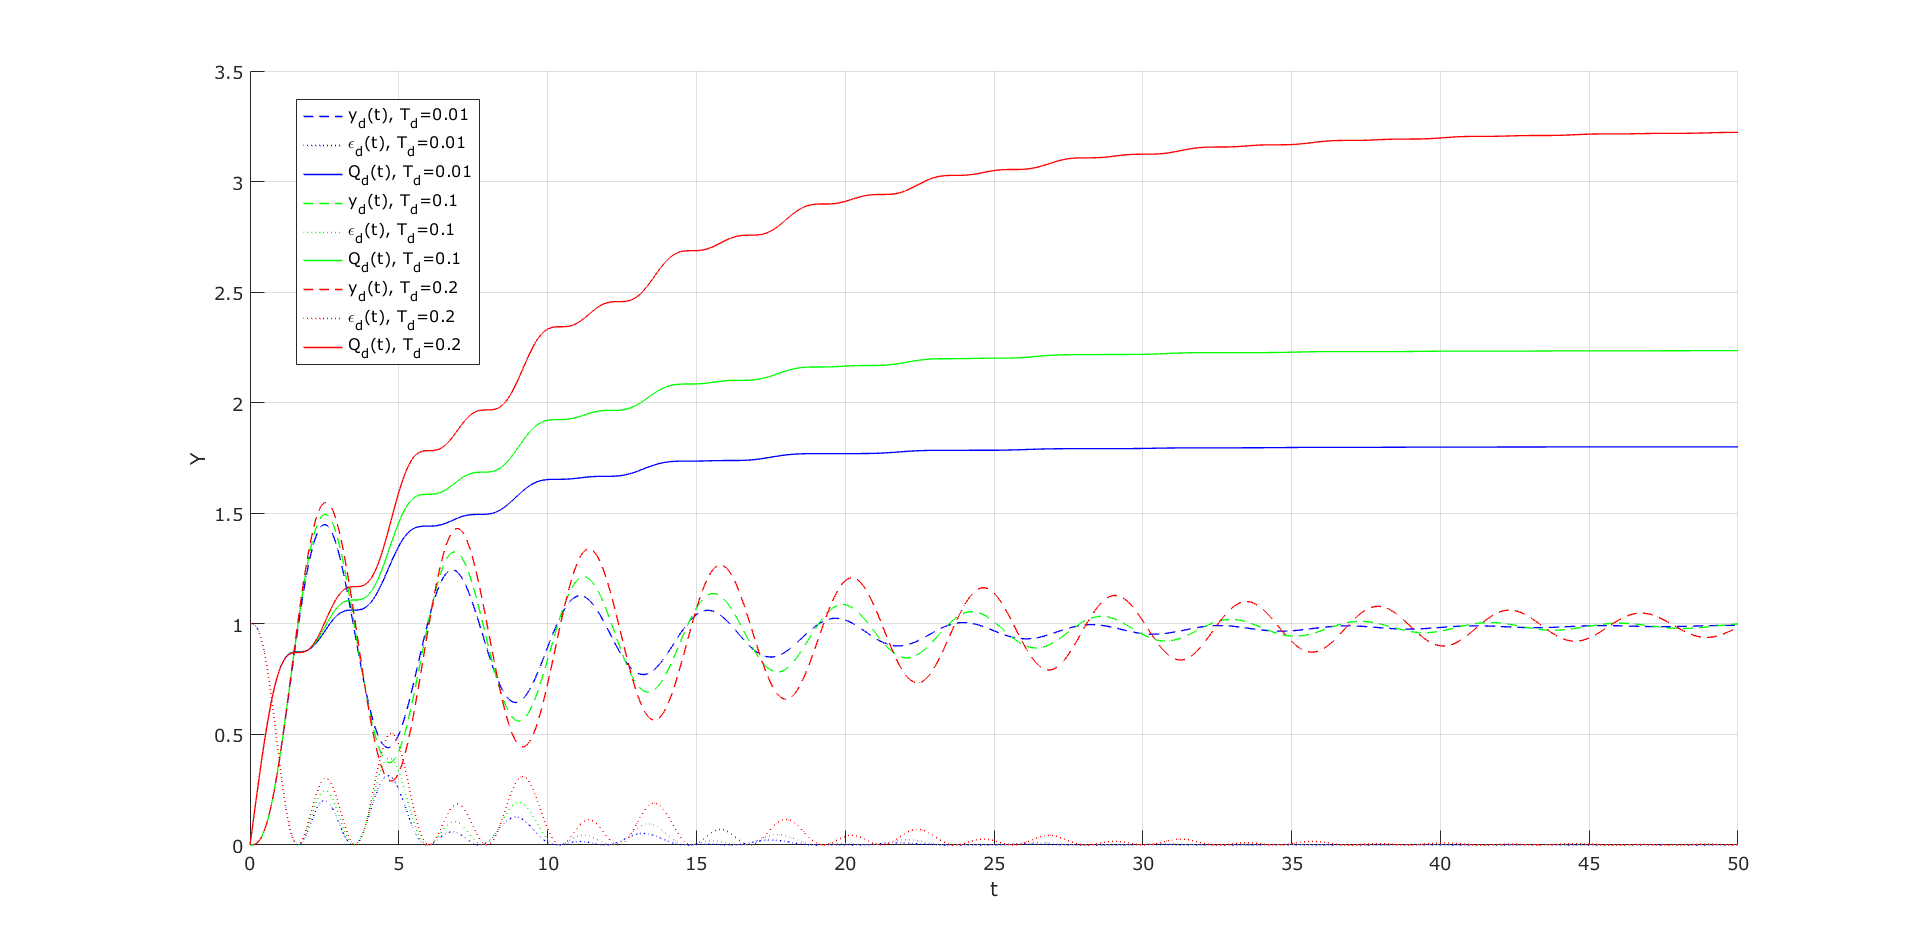
\includegraphics{3_2.png}}
\caption{Układ z regulacją dyskretną dla róźnych okresów impulsowania \(T_d\)}
\end{figure}

Z rysunku 4 widać, że odpowiedź UAR z regularorem dyskretnym jest zbliżona do UAR z regulatorem ciągłym, ale nie taka sama.

\subsection{Sterowanie odcinkami}

\begin{figure}[ht]
\centering
\scalebox{0.15}{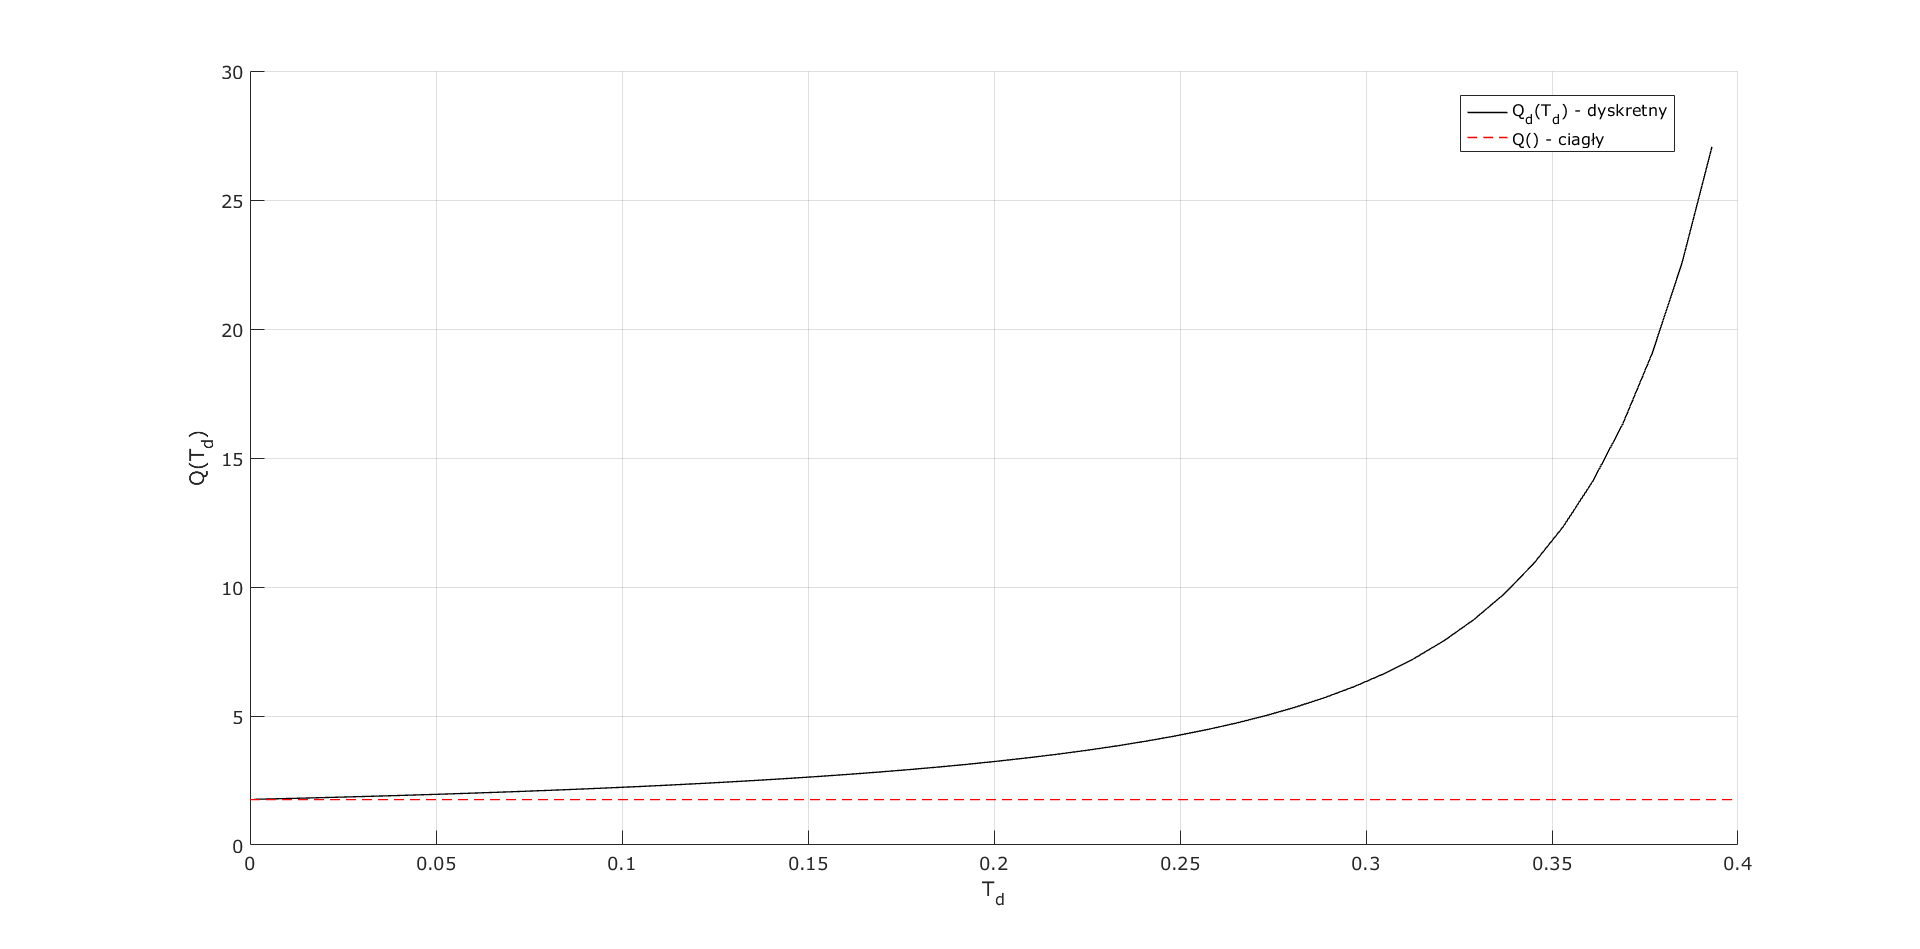
\includegraphics{3_3.png}}
\caption{Zależność \( Q_d = \int_{0}^{100} \epsilon(t)^2  dt\ \) od \(T_d\)}
\end{figure}

\section{Wnioski}


Układ dyskretnty jest tym bardziej zbliżony do ciagłego, im większa jest jego częstotliwość próbkowania na wejściu. W danym UAR przy zwiększeniu okresu próbkowania \(T_d\) wzrastał czas na stablilizacji układu, a po przekroczeniu \(T_d\) pewnej wartości UAR zamieniał się w niestabilny.
\par
Dyskretyzacja układu regulacji ciągłej może być wykorzystana do modelowania, optymalizacji i badania zachowania sterownika cyfrowego na obiekcie fizycznym w czasie ciągłym w warunkach przybliżonych do rzeczywistych.

\end{document}


